\section{信号提取}
为提取信号数目,本论文采用了质量-寿命联合拟合技术。针对质量部分,信号用双Crystal Ball(CB)函数~\cite{Skwarnicki:1986xj}来描述。
其定义如下:
\begin{equation}
 f_{\mathrm{CB}}(m;\mu,\sigma,\alpha,n) = 
 \begin{cases} 
      \Big(\frac{n}{|\alpha|}\Big)^n e^{-\frac{1}{2}\alpha^2} (\frac{n}{|\alpha|}-|\alpha|-\frac{m-\mu}{\sigma})^{-n} & \frac{m-\mu}{\sigma} < -|\alpha|\\
   \exp\Bigg( -\frac{1}{2}\Big(\frac{m-\mu}{\sigma}\Big)^2\Bigg) & \frac{m-\mu}{\sigma}>-|\alpha|.
\end{cases},
\end{equation}
CB函数是由一个高斯函数的核心(通过参数 $\mu$和$\sigma$描述)和一个左端的用来描述初态辐射效应的尾巴(通过参数 $\alpha$和$n$描述)构成。
在拟合的时候并不是所有的参数都是浮动的我们固定了其中的一些参数或者参数与参数直接的关系(这些值大多通过MC研究固定)。
比如,两个CB函数共享同一个$\mu$值,但是宽度不同,分别为$\sigma_1$和$\sigma_2$。
但是$\sigma_1$和$\sigma_2$直接具有固定的关系,即,$\sigma_2=25.7+\sigma_1$。
此外,通过MC模拟,我们将两个CB函数之间的相对比例固定为0.96.
$n$固定到了1,
$\alpha$和$\sigma$直接具有关系$\alpha=2.066\pm0.0085\sigma-0.00011\sigma^2$(此处只两个CB函数各自的$\alpha$和$\sigma$都具有同样的关系)。
因此在最终的拟合里面,只要$\mu$ 和 $\sigma_1$是浮动的。
对于质量谱上的本底成分采用指数函数$f_{\rm bkg}(m)=a_0e^{-p_0\,m}$来描述。

针对$t_{z}$的描述,$\pp$对撞直接产生的$\psitwos$ 介子信号用一个$\delta(t_z)$ 函数描述,$b$强子飞行一段时间衰变产生的$\psitwos$介子信号用指数函数描述。
因为数据是经过了探测器重建的,所以两个信号过程应该都要卷积一个分辨函数之后才能描述数据。
分辨函数用两个高斯来描述,其参数化形式如下:
\begin{equation}
f_\mathrm{resolution}(t_z;\mu,S_1,S_2,\beta) = \frac{\beta}{\sqrt{2\pi}S_1\sigma} e^{-\frac{(t_z-\mu)^2}{2S_1^2\sigma^2}}
+\frac{1-\beta}{\sqrt{2\pi}S_2\sigma} e^{-\frac{(t_z-\mu)^2}{2S_2^2\sigma^2}}.
\end{equation}
参数$\sigma$我们取自数据中$t_z$的重建误差,是逐个事例计算的。
另外一种情况我们也需要考虑到``wrong" PV事例,这指的是该事例本身是真正的$\psitwos$,但是由于重建效率的原因,个别事例的PV没有正确重建出来,从而指定了一个错误的PV。
这类事例的$t_z$分布会拖着一个较长的尾巴。
这种事例我们通过数据中故意将PV搞错来重新计算$t_z$,从而拿到他们的形状。
具体做法是在当前事例的$t_z$重建过程中使用下一个事例的PV信息来进行计算。 即,
\begin{equation}
t_z^\mathrm{next}=\frac{(z_{\mu\mu}-z_\mathrm{PV}^\mathrm{next})\times m_{\mu\mu}}{p_z},
\end{equation}
由于$\lhcb$非常好的顶点重建能力,这种事例其实非常之少。


$t_{z}$本底用一个$\delta$ 函数加多个指数函数的经验公式~\ref{eq:TzBKG}来描述,本底参数值通过拟合质量谱的边带区域进行了固定。
质量谱的边带区选择为$3566<m_{\mumu}<3620\mevcc$和$3750<m_{\mumu}<3806\mevcc$的区域。
\begin{align}
f_\mathrm{background} &=
\left[(1-f_1-f_2-f_3-f_4)\delta(t_z)+\theta(t_z)(\frac{f_1}{\tau_1}e^{-t_z/\tau_1}+\frac{f_2}{\tau_2}e^{-t_z/\tau_2})\right.
\nonumber\\
&\left. +\theta(-t_z)\frac{f_3}{\tau_3}e^{t_z/\tau_3}+\frac{f_4}{2\tau_4}e^{-|t_z|/\tau_4}
\right]\ast \left(\frac{\beta'}{\sqrt{2\pi}S^{'}_1\sigma} e^{-\frac{(t_z-\mu)^2}{2S^{'2}_1\sigma^2}}
  +\frac{1-\beta'}{\sqrt{2\pi}S^{'}_2\sigma} e^{-\frac{(t_z-\mu)^2}{2S^{'2}_2\sigma^2}}\right). 
\label{eq:TzBKG}
\end{align}

%%%%%%%%%%%%%%%%%%%%%%%%%%%%%%%%%%%%%%%%%%%%%%%%%%%%%%%%%%
所以,最终对于$t_z$的拟合函数形式为:
\begin{align}
F_{t_z}(t_z;n_{\mathrm{prompt}},n_{tail},n_{\mathrm{bdecay}},n_\mathrm{bkg},\mu,S_1,S_2,\beta,\tau_b)&   \nonumber \\
      =\left(n_{\mathrm{prompt}}\delta(t_z)+\frac{n_{\mathrm{bdecay}}}{\tau_b}e^{-t_z/\tau_b}\right)\ast f_\mathrm{resolution}(t_z;\mu,S_1,S_2,\beta)
      &+n_{\mathrm{tail}} f_\mathrm{tail}(t_z)+n_\mathrm{bkg}f_\mathrm{background}(t_z), \label{eq:FinalTz}
\end{align}
其中$n_\mathrm{bkg}$, $n_{\mathrm{prompt}}$, $n_{\mathrm{bdecay}}$ 和 $n_{\mathrm{tail}}$ 指的分别是本底事例数,直接产生的$\psitwos$信号, 来自$b$强子衰变的$\psitwos$信号数以及wrong PV事例数。

图~\ref{fig:tzmass}展示了动力学区间$2<\pt<3\gevc$,$3.5<y<4.0$范围内的质量-寿命联合拟合图。
其中蓝色代表$\pp$ 对撞直接产生的$\psitwos$ 介子的分布, 黑色代表$b$强子飞行一段时间后产生的$\psitwos$介子的分布,绿色代表本底分布,红色代表总的分布。
在二维拟合过程中,质量谱拟合形状的参数$\mu_{mass}$, $\sigma_{mass}$, $p_{0}$,通过对一维的质量谱拟合进行了固定。
所有的拟合参数我们放在了附录~\ref{sec:FitResult}中的表~\ref{tab:FitResults0}-表\ref{tab:FitResults4}。

 %%%%%%%%%%%%%%%%%%%%%%%%%%%%%%%%%%%%%%%%%%%%%%%%%%%%%%%%%%%
\begin{figure}[!tbp]
\centering
\begin{minipage}[t]{0.49\textwidth}
\centering
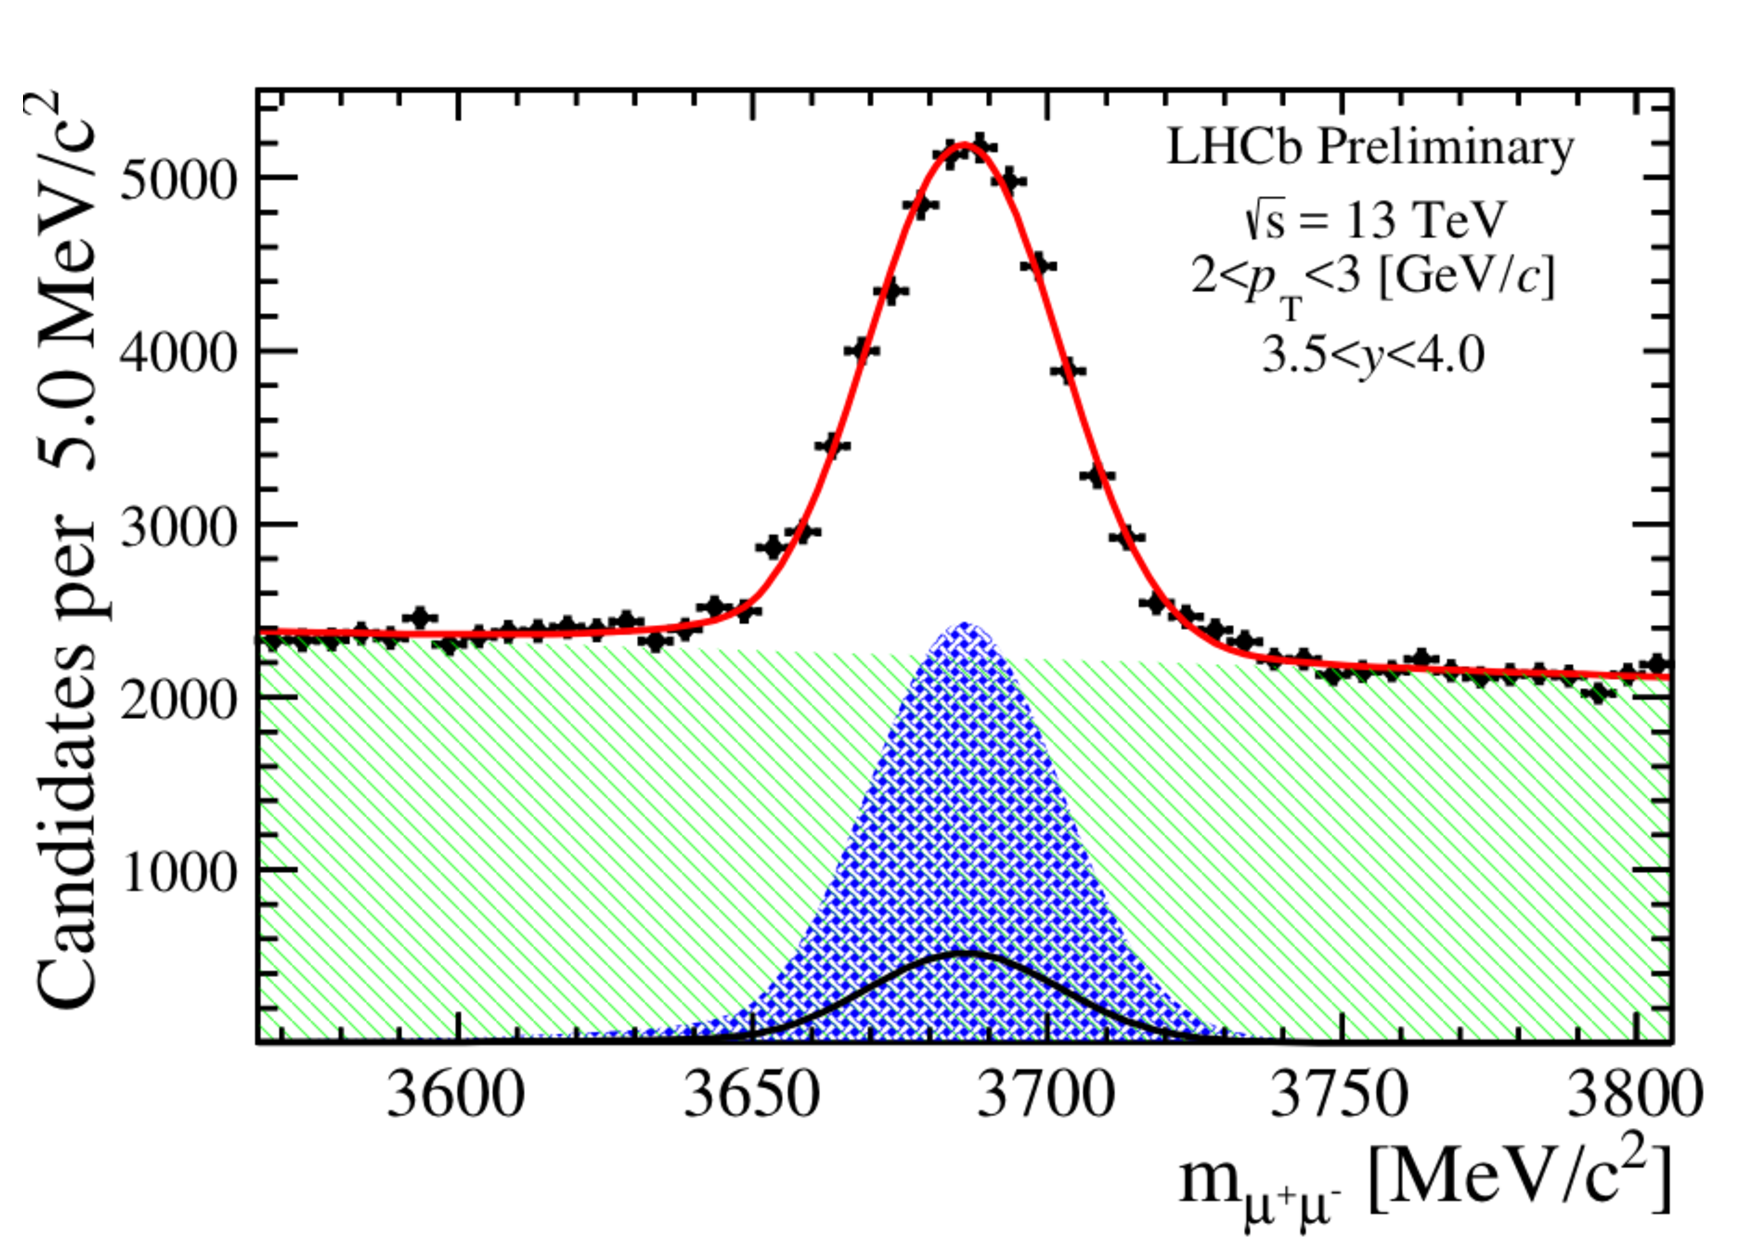
\includegraphics[width=1.0\textwidth]{chap3_fit2D_mass_3_0}
\end{minipage}
\begin{minipage}[t]{0.49\textwidth}
\centering
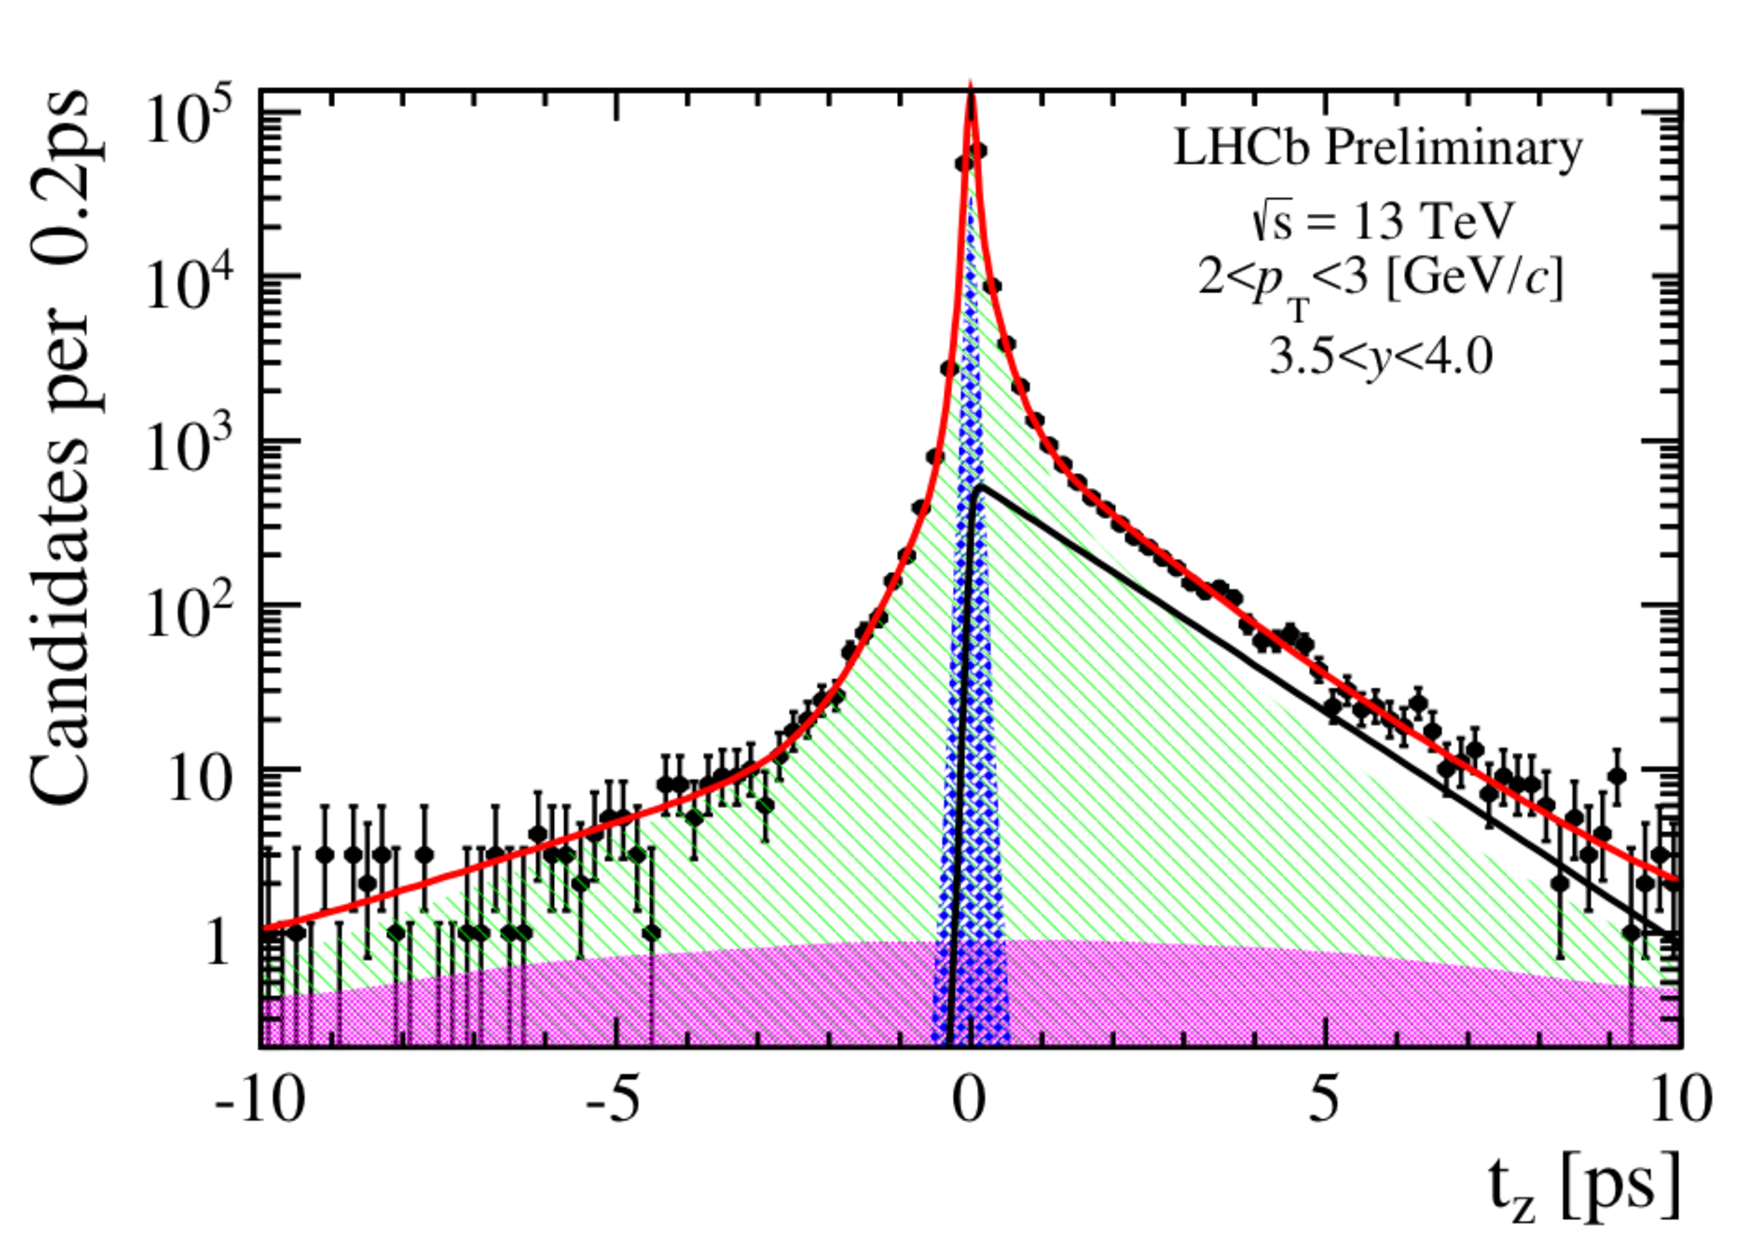
\includegraphics[width=1.0\textwidth]{chap3_fit2D_tz_3_0}
\end{minipage}
\caption{在$\psitwos$运动学区间$2<\pt<3\gevc$, $3.5<y<4.0$内的不变质量拟合分布(左图)和赝寿命拟合分布(右图)。红色的实线为总的拟合函数。绿色区域为本底。蓝色的交叉虚线区域为直接产生的$\psitwos$,黑色的为来自$b$强子衰变的$\psitwos$介子。紫色区域为wrong PV事例的分布,由于量很少,在质量谱上小到看不到了。}
\label{fig:tzmass}
\end{figure}


